\documentclass{article}
\usepackage{tikz}

\begin{document}
%~~~~~~~~~~~~~~~~~~~~~~~~~~~~~~~~~~~~~~~~
% ELEC 467 Electric Machines and Transformers
% Single Phase Transformer Initial Diagram(s)
% Written by Sze "Ron" Chau, November 2014
%~~~~~~~~~~~~~~~~~~~~~~~~~~~~~~~~~~~~~~~
% Fill color on in-between areas:
% Draw one rectangle clockwise, 
% reverse for the other
%~~~~~~~~~~~~~~~~~~~~~~~~~~~~~~~~~~~~~~~~
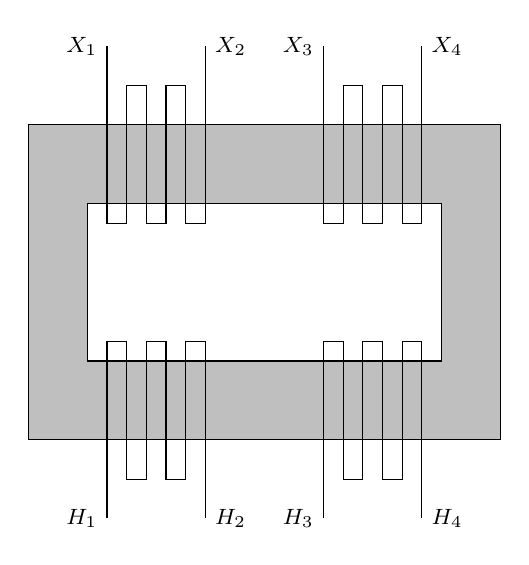
\begin{tikzpicture}

% transformer
\filldraw[fill=gray!50!white,draw=black]
    (0,0)    -- (0,4)    -- (6,4)    -- (6,0)    -- cycle
    (0.75,1) -- (5.25,1) -- (5.25,3) -- (0.75,3) -- cycle;

% H windings
\foreach \h in {1,3.75}
    \draw(\h,-1)           -- (\h,1.25) -- 
         (\h + 0.25,1.25)  -- (\h + 0.25,-0.5) -- 
         (\h + 0.5,-0.5)   -- (\h + 0.5,1.25) -- 
         (\h + 0.75,1.25)  -- (\h + 0.75,-0.5) -- 
         (\h + 1,-0.5)     -- (\h + 1,1.25) -- 
         (\h + 1.25,1.25)  -- (\h + 1.25,-1)
;
    
% X windings
\foreach \ns in {1,3.75}
    \draw(\ns,5)           -- (\ns,2.75) -- 
         (\ns + 0.25,2.75) -- (\ns + 0.25,4.5) -- 
         (\ns + 0.5,4.5)   -- (\ns + 0.5,2.75) -- 
         (\ns + 0.75,2.75) -- (\ns + 0.75,4.5) -- 
         (\ns + 1,4.5)     -- (\ns + 1,2.75) -- 
         (\ns + 1.25,2.75) -- (\ns + 1.25,5)
;

% labels    
\draw (1,-1)    node[anchor=east]{\footnotesize $H_{1}$};
\draw (2.25,-1) node[anchor=west]{\footnotesize $H_{2}$};
\draw (3.75,-1) node[anchor=east]{\footnotesize $H_{3}$};
\draw (5,-1)    node[anchor=west]{\footnotesize $H_{4}$};
\draw (1,5)     node[anchor=east]{\footnotesize $X_{1}$};
\draw (2.25,5)  node[anchor=west]{\footnotesize $X_{2}$};
\draw (3.75,5)  node[anchor=east]{\footnotesize $X_{3}$};
\draw (5,5)     node[anchor=west]{\footnotesize $X_{4}$};

\end{tikzpicture}
\end{document}